\documentclass[smallextended,envcountsect]{svjour3}

\usepackage{amsmath,amssymb,amsfonts,mathtools}
\usepackage{graphicx}
\usepackage{booktabs}
\usepackage{url}
\usepackage[hidelinks]{hyperref}
\hypersetup{
  pdftitle={Dimension-Free Loss-Landscape Barrier Decay via Atomic Self-Sparsification},
  pdfauthor={Saveliy Baturin},
  pdfkeywords={nonconvex optimization, loss landscape, sublevel-set connectivity,
    ReLU networks, overparameterization}
}

\smartqed
\journalname{Journal of Optimization Theory and Applications}
\spnewtheorem{assumption}{Assumption}[section]{\bfseries}{\rmfamily}
\let\jotaendproof\endproof
\renewcommand{\endproof}{\qed\jotaendproof}
\newcommand{\doi}[1]{\href{https://doi.org/#1}{\nolinkurl{https://doi.org/#1}}}

\newcommand{\relu}{\operatorname{ReLU}}
\newcommand{\E}{\mathbb{E}}
\newcommand{\R}{\mathbb{R}}
\newcommand{\norm}[1]{\left\lVert #1 \right\rVert}
\newcommand{\abs}[1]{\left\lvert #1 \right\rvert}
\newcommand{\inner}[2]{\left\langle #1,#2 \right\rangle}
\newcommand{\SigX}{\Sigma_X}
\newcommand{\supp}{\operatorname{supp}}
\newcommand{\SubBar}{\mathfrak b}

\raggedbottom
\setlength{\emergencystretch}{2em}

\begin{document}

\title{Dimension-Free Loss-Landscape Barrier\\
Decay via Atomic Self-Sparsification}

\author{Saveliy Baturin}

\institute{Saveliy Baturin, Corresponding Author \at
Independent Researcher\\
Russia\\
\email{saveliy.xo@gmail.com}}

\date{}

\begingroup
\hfuzz=0.5pt % svjour3 title-box rounding (0.37035 pt)
\maketitle
\endgroup

\begin{abstract}
We study pathwise connectivity of regularized-risk sublevel sets for shallow
rectified-linear neural networks. The central construction sparsifies each
endpoint on its own fixed dictionary. Sampling atoms proportionally to
output-layer mass preserves the variation penalty, is unbiased in function
space, and frees a prescribed number of neurons without moving their
first-layer directions. Combining these compressed endpoints with a common
sparse reference network yields dimension-independent barrier bounds uniformly
over all pairs in a bounded sublevel. For convex globally Lipschitz losses,
barriers for bounded moving levels decay at an inverse-square-root rate, whereas
smallest-mass pruning gives an inverse-linear rate at every fixed level above
the limiting objective. When the loss derivative is H\"older continuous, the
moving-level rate improves with smoothness and becomes inverse-linear when the
derivative is Lipschitz. A function-preserving balancing deformation transfers
all fixed- and moving-level bounds to the raw parameters of standard two-layer
quadratic weight decay. The same estimates give a connected-component merge
interpretation under sublevel inclusion. Finite-distribution diagnostics verify
the sampling law, smooth-loss cancellation, balancing invariants, and the
complete zero-buffer path, while remaining separate from the worst-case
theoretical claims.
\end{abstract}

\keywords{Nonconvex optimization \and Loss landscape \and
Sublevel-set connectivity \and ReLU networks \and Overparameterization}

\subclass{41A25 \and 68T07 \and 90C26}

\section{Introduction}\label{sec:introduction}

The objective of this paper is a quantitative question about a specific nonconvex model: how much must the regularized risk increase when two parameter points in the same sublevel set are joined by a continuous path?  The answer is expressed through an approximation quantity of the underlying shallow-network class.

Freeman and Bruna \cite{FreemanBruna2017} proved an asymptotic connectivity mechanism for half-rectified one-hidden-layer networks with quadratic loss. Their argument combines output-layer convexity, sparse compression, and clusters of nearby first-layer directions. The resulting rate inherits the covering dimension of the atom space. We retain the compression--relocation architecture but remove its geometric bottleneck: each endpoint is compressed on its own fixed dictionary, by unbiased sampling or smallest-mass pruning. The atom locations never move during compression, so the exponent no longer depends on input dimension.

The parameter constraint needs particular care. Positive homogeneity gives
\[
 a\relu(w^\top x)=\frac{a}{c}\relu((cw)^\top x),\qquad c>0,
\]
but this rescaling changes an $\ell_1$ penalty imposed only on $a$. Consequently, normalizing the first layer is not a harmless ``without loss of generality'' operation. We formulate the model on a product of closed Euclidean unit balls. This is a genuine architectural constraint, and its convexity ensures that the first-layer interpolations used below remain admissible.

The main contributions are the following.
\begin{enumerate}
\item We prove an attained finite-width master bound and a zero-radius path principle that converts any penalty-compatible endpoint compression into a path through a common reference network.
\item We introduce penalty-preserving self-sparsification on each endpoint's
fixed dictionary. It yields $O(m^{-1/2})$ moving-level thickening for convex
Lipschitz losses. A smallest-mass pruning argument gives $O(m^{-1})$ at every
fixed level above $e_\infty$, uniformly over arbitrary sublevel endpoints and
in every input dimension.
\item For losses with $\alpha$-H\"older derivative, unbiasedness cancels the first-order Taylor term and improves both objective approximation and moving-level barriers to $O(m^{-(1+\alpha)/2})$. The smooth endpoint includes half-squared error, Huber loss, and binary cross-entropy in logits.
\item We define the raw-parameter barrier for two-layer quadratic weight decay
and prove the same fixed- and moving-level rates through a filtered balancing
retraction. As a topological interpretation, the barrier bound also controls
the merge scale of reduced $H_0$ classes.
\item We give theorem-aligned diagnostics for random self-sparsification and
smooth first-order cancellation up to input dimension 128. They also check the
balancing lift and retain a separate complete-path stress test.
\end{enumerate}

The asymptotic results concern the evolution of the approximation class with width; they are not convergence theorems for gradient descent or claims about training-time dynamics. The $q^{-1/2}$ and $q^{-1}$ fixed-dictionary function-approximation orders cannot be improved under only a bounded-atom envelope, but neither ReLU-dictionary nor barrier sharpness is claimed. Apart from the explicit one-dimensional and strong-regularization cases, the paper does not assert exact finite-width population connectivity or make a statement about ordinary dense deep networks.

Throughout, width means the number of hidden neurons, and a sublevel barrier is
the least objective increase needed to join two points at a prescribed
regularized-risk level. Precise notation is introduced in
Section~\ref{sec:setting}. The remainder of this introduction reviews the
closest connectivity, convex-reformulation, and approximation results.
Section~\ref{sec:finite} proves the finite-width master bound,
Section~\ref{sec:rates} develops self-sparsification and dimension-free rates,
Section~\ref{sec:weight-decay} transfers them to ordinary weight decay,
Section~\ref{sec:computational} reports the diagnostics, and
Section~\ref{sec:discussion} discusses scope and limitations.

\subsection{Sublevel-Set Topology}\label{sec:related}
The closest point of departure is Freeman and Bruna \cite{FreemanBruna2017}. For a regularized half-rectified shallow model with quadratic loss, they bound the excess energy of a path through a sparse-approximation functional and a perturbation of hidden directions, and then obtain asymptotic connectivity from a covering argument. Our finite-width master construction retains their compression--relocation logic. The main rates, however, use no direction perturbation: fixed-dictionary sampling and pruning supply zero-radius bridges. This distinction removes the atom-space covering exponent.

Venturi, Bandeira, and Bruna \cite{Venturi2019} characterize spurious valleys of one-hidden-layer objectives through intrinsic dimension, whereas Nguyen \cite{Nguyen2019} proves exact connectedness of every empirical-loss sublevel for sufficiently overparameterized piecewise-linear deep networks under sample-size-dependent width conditions. These are exact or qualitative topology results under assumptions different from ours. Simsek et al.\ \cite{Simsek2021} instead describe connected manifolds of global minima generated by overparameterization and permutation symmetry. Our object is neither only the minimizer set nor a sample-size width threshold: it is the worst excess along paths between arbitrary points of a prescribed regularized-risk sublevel.

Nurisso, Leroy, and Vaccarino \cite{Nurisso2024} identify disconnected components of the quadric invariant sets imposed on shallow ReLU gradient flow by homogeneity. Their subsequent DAG-architecture analysis with Petri \cite{Nurisso2026} characterizes connectedness and singularities of the corresponding training-invariant learning spaces. This is complementary to our result: they study reachability constrained by gradient-flow conservation laws, whereas our paths range over the full constrained parameter sublevel and are not asserted to be optimization trajectories. Wu, Simsek, and Ged \cite{Wu2025} analyze directional stationary points, saddle escape, and width embeddings for shallow ReLU-like networks with empirical squared loss; our theorem instead concerns arbitrary sublevel endpoints and convex globally Lipschitz losses.

\subsection{Approximate Connectivity and Trained Solutions}
Kuditipudi et al.~\cite{Kuditipudi2019} explain low-cost piecewise-linear connections from dropout and noise stability of trained networks. Shevchenko and Mondelli \cite{ShevchenkoMondelli2020} make the width dependence explicit and dimension-free for two-layer SGD solutions. Mean-field particle analyses also give dimension-free finite-width approximation orders along selected dynamics \cite{RotskoffVandenEijnden2022}. Ferbach et al.~\cite{Ferbach2024} give a different probabilistic explanation through Wasserstein convergence and alignment. These results condition on properties, distributions, or dynamics of trained solutions. Here no training algorithm appears and the endpoints are arbitrary elements of an entire bounded regularized sublevel.

\subsection{Convex Reformulations}
Convex reformulations expose additional structure in regularized two-layer ReLU training. Standard weight decay is equivalent to a block-$\ell_1$ convex regularizer on a finite dataset \cite{PilanciErgen2020}. Wang, Lacotte, and Pilanci construct paths from networks to structured representatives and characterize widths without spurious valleys \cite{WangLacottePilanci2022}; Mishkin and Pilanci characterize optimal sets and pruning paths \cite{MishkinPilanci2023}. Kim, Mishkin, and Pilanci use convex duality to characterize width-dependent connectivity of regularized optimal sets and construct non-increasing paths toward globally optimal representations \cite{KimMishkinPilanci2025}. Our claim is therefore not a new finite-sample Carath\'eodory theorem. It is a quantitative population-risk bound uniform over arbitrary endpoints, with no sample-size threshold.

\subsection{Empirical Mode Connectivity}
Low-loss paths between independently trained networks were first constructed at scale by Draxler et al.\ and Garipov et al.\ \cite{Draxler2018,Garipov2018}. A later line of work asks whether much simpler linear paths emerge after quotienting neuron-permutation symmetries. Entezari et al.\ \cite{Entezari2022} formulated and empirically tested the permutation-invariance conjecture; Ainsworth et al.\ \cite{Ainsworth2023} developed weight-matching algorithms for model merging; and Jordan et al.\ \cite{Jordan2023} showed that activation-variance collapse can remain after alignment and proposed a renormalization repair. More recently, Zhao et al.\ \cite{Zhao2025} related mode connectivity to continuous parameter symmetries and derived explicit symmetry-induced connecting curves. This literature concerns trained modes, alignment, and often deep architectures. It motivates the direct-interpolation baseline in Section~\ref{sec:computational}, but does not imply the uniform sublevel theorem proved here; conversely, our theorem neither identifies permutation alignments nor claims linear connectivity.

\subsection{Approximation Theory}
Quantitative approximation by neural networks has a long history; representative entry points include Barron's sampling bounds \cite{Barron1993} and Pinkus's survey of multilayer perceptron approximation \cite{Pinkus1999}. Recent work develops optimal rates and lower bounds for shallow ReLU variation spaces \cite{YangZhou2025,Siegel2025}; convex Lipschitz losses also appear in contemporary constructive-approximation analyses of kernel approximations \cite{Lian2026}. Our approximation statement has a different purpose. Rather than posit a target-class norm, Lemma~\ref{lem:maurey} sparsifies near-minimizers of the exact regularized objective. The sampling primitive is classical in spirit; the contribution is its uniform transfer from every bounded-sublevel endpoint to quantitative sublevel topology, including the smooth first-order cancellation.

\section{Model and Quantities}\label{sec:setting}

Let
\[
B_2^n=\{w\in\R^n:\norm{w}_2\le 1\},
\qquad
\mathcal W_m=(B_2^n)^m\times\R^m.
\]
For $\vartheta=(W,\theta)\in\mathcal W_m$, where the rows of $W$ are $w_1,\ldots,w_m$, define
\begin{equation}
\Phi_m(x;W,\theta)
=\sum_{i=1}^m\theta_i\relu(w_i^\top x).
\label{eq:model}
\end{equation}
The first-layer ball constraint is part of the model. In particular, the objective below would be ill posed under unrestricted positive rescaling of $W$ with a penalty only on $\theta$.

Let $(X,Y)$ have distribution $P$, and let
\begin{equation}
R_m(W,\theta)
=\E\!\left[\mathcal L\!\left(Y,\Phi_m(X;W,\theta)\right)\right],
\qquad
F_m(W,\theta)=R_m(W,\theta)+\kappa\norm{\theta}_1,
\label{eq:objective}
\end{equation}
where $\kappa>0$. Write $\SigX=\E[XX^\top]$ and
\[
D_X=\sqrt{\norm{\SigX}_{\mathrm{op}}}.
\]

\begin{assumption}[Lipschitz regime]\label{ass:standing}
The second moment of $X$ is finite, and $\E[\abs{\mathcal L(Y,0)}]<\infty$. For $P_Y$-almost every $y$, the map $u\mapsto\mathcal L(y,u)$ is convex and $L$-Lipschitz, with the same finite constant $L$. There is a finite constant $\underline R$ such that
\[
R_m(W,\theta)\ge \underline R
\]
for every width $m$ and every $(W,\theta)\in\mathcal W_m$.
\end{assumption}

For example, binary cross-entropy with a scalar logit $u$ and label $y\in\{0,1\}$ is
\begin{equation}
\mathcal L_{\rm BCE}(y,u)=\log(1+e^u)-yu.
\label{eq:bce-logit}
\end{equation}
It is convex and globally $1$-Lipschitz in the logit because
$\partial_u\mathcal L_{\rm BCE}(y,u)=\sigma(u)-y\in[-1,1]$.
Thus no bounded-logit assumption is needed. Quadratic loss is treated below by the alternative smooth-loss assumption.

\begin{definition}[Sublevel and pairwise barrier]
For $\lambda\in\R$, set
\[
\Omega_m(\lambda)=\{\vartheta\in\mathcal W_m:F_m(\vartheta)\le\lambda\}.
\]
For $\vartheta^A,\vartheta^B\in\mathcal W_m$, define
\begin{equation}
\operatorname{bar}_m(\vartheta^A,\vartheta^B)
=\inf_{\gamma}\left(
\max_{t\in[0,1]}F_m(\gamma(t))
-\max\{F_m(\vartheta^A),F_m(\vartheta^B)\}
\right),
\label{eq:pair-barrier}
\end{equation}
where the infimum is over continuous paths in $\mathcal W_m$ with the prescribed endpoints.
\end{definition}

For a uniform sublevel statement it is convenient to measure thickening above the specified level, rather than above the individual endpoint values.

\begin{definition}[Sublevel thickening]\label{def:thickening}
Define
\begin{equation}
\SubBar_m(\lambda)
=\sup_{\vartheta^A,\vartheta^B\in\Omega_m(\lambda)}
\inf_{\gamma}
\left(\max_{t\in[0,1]}F_m(\gamma(t))-\lambda\right)_+.
\label{eq:thickening}
\end{equation}
If the sublevel is empty, the supremum is set to zero.
\end{definition}

The approximation values used below are
\begin{equation}
e(l)
=\min_{(U,\xi)\in\mathcal W_l}F_l(U,\xi),
\qquad
e_\infty=\lim_{l\to\infty}e(l).
\label{eq:e-l}
\end{equation}
The limit exists because $e(l)$ is nonincreasing: an $l$-neuron model embeds into width $l+1$ by adding a zero output coefficient.

For $W\in(B_2^n)^m$, an active-neuron budget $q\le m$, and $r\ge0$, define the loss-consistent robust compression value
\begin{equation}
\delta_W^{\mathcal L}(q,r;m)
=\min_{\substack{\gamma\in\R^m,\ \norm{\gamma}_0\le q\\
\widehat W\in(B_2^n)^m,\ \max_i\norm{\hat w_i-w_i}_2\le r}}
F_m(\widehat W,\gamma).
\label{eq:delta}
\end{equation}
Unlike an angular definition on the sphere, \eqref{eq:delta} is compatible with convex interpolation inside the parameter domain.

\begin{lemma}[Attainment and output-layer control]\label{lem:attainment}
Under Assumption~\ref{ass:standing}, or under the common moment assumptions together with Assumption~\ref{ass:holder} stated in Section~\ref{sec:rates}, the minima in \eqref{eq:e-l} and \eqref{eq:delta} are attained. Moreover,
\begin{equation}
F_m(W,\theta)\le s
\quad\Longrightarrow\quad
\norm{\theta}_1\le\frac{s-\underline R}{\kappa}.
\label{eq:l1-control}
\end{equation}
where one takes $\underline R=0$ in the nonnegative H\"older-smooth regime.
\end{lemma}

\begin{proof}
The implication \eqref{eq:l1-control} follows from
\[
s\ge R_m(W,\theta)+\kappa\norm{\theta}_1
\ge\underline R+\kappa\norm{\theta}_1.
\]
For attainment, take a minimizing sequence. Its objective values are bounded above, so \eqref{eq:l1-control} bounds its output coefficients. The first-layer variables range over a compact set, and the sparsity constraint in \eqref{eq:delta} is a finite union of closed coordinate subspaces. The additional rowwise distance constraint in \eqref{eq:delta} is closed. Hence a convergent subsequence $(W_j,\theta_j)\to(W,\theta)$ exists. On a set where the output coefficients are bounded, the ReLU inequality
\[
\E\abs{\relu(a^\top X)-\relu(b^\top X)}
\le D_X\norm{a-b}_2
\label{eq:relu-lipschitz}
\]
gives the explicit joint bound
\[
\begin{aligned}
&\E\abs{\Phi_m(X;W_j,\theta_j)-\Phi_m(X;W,\theta)}\\
&\qquad\le D_X\norm{\theta_j-\theta}_1
   +D_X\norm{\theta}_1\max_i\norm{w_{j,i}-w_i}_2,
\end{aligned}
\]
because every first-layer row has norm at most one. The right-hand side tends to zero. In the Lipschitz regime this implies continuity of the expected risk.
In the H\"older-smooth regime, the same predictor estimate holds in $L^2(P_X)$ and hence in $L^{1+\alpha}(P_X)$. The descent estimate \eqref{eq:holder-descent}, applied at zero, implies
\[
 \abs{\partial_u\mathcal L(Y,0)}^{(1+\alpha)/\alpha}
 \le \frac{1+\alpha}{\alpha}H^{1/\alpha}\mathcal L(Y,0).
\]
Together with
$\abs{\partial_u\mathcal L(Y,u)}\le
\abs{\partial_u\mathcal L(Y,0)}+H\abs u^\alpha$,
H\"older's inequality gives continuity of the expected risk on every bounded parameter set. The $\ell_1$ term is continuous in finite dimension, so the subsequential limit attains the infimum in either regime.
\end{proof}

\section{A Finite-Width Path Bound}\label{sec:finite}

We first isolate the perturbation step that replaces the quadratic estimate.

\begin{lemma}[Lipschitz bridge]\label{lem:bridge}
Let $(W,\beta),(\widehat W,\gamma)\in\mathcal W_m$ satisfy
\[
\max_i\norm{w_i-\hat w_i}_2\le r,
\qquad
F_m(W,\beta)\le\Lambda,
\qquad
F_m(\widehat W,\gamma)\le\Lambda.
\]
Then the path
\[
W_t=(1-t)W+t\widehat W,
\qquad
\theta_t=(1-t)\beta+t\gamma
\]
lies in $\mathcal W_m$ and satisfies
\begin{equation}
F_m(W_t,\theta_t)
\le
\Lambda+\frac{LD_X}{\kappa}r(\Lambda-\underline R),
\qquad 0\le t\le1.
\label{eq:bridge-bound}
\end{equation}
\end{lemma}

\begin{proof}
The unit ball is convex, so every row of $W_t$ is admissible. Introduce the extended convex logit
\[
g_t(X)=(1-t)\Phi_m(X;W,\beta)
+t\Phi_m(X;\widehat W,\gamma).
\]
Convexity of the loss and of the $\ell_1$ norm gives
\begin{equation}
\E[\mathcal L(Y,g_t(X))]
+\kappa\big((1-t)\norm{\beta}_1+t\norm{\gamma}_1\big)
\le\Lambda.
\label{eq:extended-convex}
\end{equation}
For $w_{t,i}=(1-t)w_i+t\hat w_i$, the difference between the genuine and extended logits is
\begin{align*}
\Phi_m(X;W_t,\theta_t)-g_t(X)
={}&\sum_i(1-t)\beta_i
\bigl(\relu(w_{t,i}^\top X)-\relu(w_i^\top X)\bigr)\\
&+\sum_i t\gamma_i
\bigl(\relu(w_{t,i}^\top X)-\relu(\hat w_i^\top X)\bigr).
\end{align*}
Using \eqref{eq:relu-lipschitz}, $\norm{w_{t,i}-w_i}\le r$, and $\norm{w_{t,i}-\hat w_i}\le r$, its expected absolute value is at most
\[
rD_X\big((1-t)\norm{\beta}_1+t\norm{\gamma}_1\big).
\]
Lemma~\ref{lem:attainment} bounds both $\ell_1$ norms by $(\Lambda-\underline R)/\kappa$. Combining the Lipschitz estimate for $\mathcal L$ with \eqref{eq:extended-convex}, and using $\norm{\theta_t}_1\le(1-t)\norm{\beta}_1+t\norm{\gamma}_1$, proves \eqref{eq:bridge-bound}.
\end{proof}

\begin{theorem}[Finite-width bound]\label{thm:finite}
Assume Assumption~\ref{ass:standing}. Let $\vartheta^A=(W_A,\theta_A)$ and $\vartheta^B=(W_B,\theta_B)$ belong to $\Omega_m(\lambda)$. For every integer $1\le l\le m$ and every $r\ge0$, there is a continuous path $\gamma_{l,r}$ in $\mathcal W_m$ joining the endpoints such that
\begin{equation}
\max_{t\in[0,1]}F_m(\gamma_{l,r}(t))
\le
\Lambda_m(l,r;\lambda)
+\frac{LD_X}{\kappa}r
\bigl(\Lambda_m(l,r;\lambda)-\underline R\bigr),
\label{eq:finite-bound}
\end{equation}
where
\begin{equation}
\Lambda_m(l,r;\lambda)
=\max\!\left\{
\lambda,
e(l),
\delta_{W_A}^{\mathcal L}(m-l,r;m),
\delta_{W_B}^{\mathcal L}(m-l,r;m)
\right\}.
\label{eq:Lambda}
\end{equation}
\end{theorem}

\begin{proof}
We give the construction for the $A$ endpoint and then reverse its analogue for $B$.

First keep $W_A$ fixed and linearly interpolate $\theta_A$ to a minimizer $\beta_A$ of $\delta_{W_A}^{\mathcal L}(m,0;m)$. Both endpoints have objective at most $\lambda$, since $(W_A,\theta_A)$ is feasible in that minimization. Convexity in the logit and of the $\ell_1$ norm keeps the whole segment below $\lambda$.

Let $(\widehat W_A,\eta_A)$ attain $\delta_{W_A}^{\mathcal L}(m-l,r;m)$. Lemma~\ref{lem:bridge} connects $(W_A,\beta_A)$ to $(\widehat W_A,\eta_A)$ below the right-hand side of \eqref{eq:finite-bound}.

Let $(U^\star,\xi^\star)\in\mathcal W_l$ attain $e(l)$. Since $\eta_A$ has at most $m-l$ nonzero coordinates, at least $l$ first-layer rows carry zero output coefficients. Move those rows, at constant predictor and constant objective, to the rows of $U^\star$. With this combined first layer fixed, linearly interpolate the output vector from $\eta_A$ to the corresponding embedding of $\xi^\star$. Convexity bounds this segment by
\[
\max\{\delta_{W_A}^{\mathcal L}(m-l,r;m),e(l)\}\le\Lambda_m(l,r;\lambda).
\]

It remains to ensure that the $A$ and $B$ constructions reach the same parameter point, not merely the same predictor. If $l<m$, there is at least one zero output coordinate after the preceding interpolation. Such a coordinate is a buffer: move its first-layer row to an active row $u$, transfer a coefficient $a$ continuously by replacing $(a,0)$ with $((1-t)a,ta)$ on the two now-identical rows, and then move the newly inactive row freely. Throughout this move the predictor is identical and the penalty equals $|(1-t)a|+|ta|=|a|$. Repeating the move implements any required finite permutation and places the reference atoms in a fixed set of $l$ coordinates and a fixed order. All remaining zero-coefficient rows are then moved to the zero vector.

If $l=m$, then $m-l=0$ forces $\eta_A=\eta_B=0$. On each side all rows may therefore be moved, at constant zero predictor, directly to $U^\star$ in the same prescribed order before interpolating the output coefficients to $\xi^\star$. Thus in both cases the two one-sided constructions reach the identical labeled parameter point, namely the canonical embedding of $(U^\star,\xi^\star)$.

Concatenating the $A$ path with the reverse $B$ path proves the result.
\end{proof}

\begin{remark}[What is new in the bridge]\label{rem:novelty}
The combinatorial path architecture follows the mechanism of Freeman and Bruna \cite{FreemanBruna2017}. The loss-specific step is Lemma~\ref{lem:bridge}: global Lipschitz continuity converts a logit perturbation directly into a first-order risk perturbation. No quadratic expansion is used.
\end{remark}

\begin{lemma}[Monotone sphericalization]\label{lem:sphericalize}
Every $(W,\theta)\in\mathcal W_m$ is connected to a point $(W^\circ,\theta^\circ)\in\mathcal W_m$ such that
\begin{equation}
\theta_i^\circ\ne0
\quad\Longrightarrow\quad
\norm{w_i^\circ}_2=1,
\label{eq:spherical-active}
\end{equation}
the predictor is constant along the path, and the objective is nonincreasing. In particular,
$F_m(W^\circ,\theta^\circ)\le F_m(W,\theta)$ and
$\norm{\theta^\circ}_1\le\norm{\theta}_1$.
\end{lemma}

\begin{proof}
It is enough to treat one row at a time. If $\theta_i=0$, no move is needed. If $\theta_i\ne0$ but $w_i=0$, linearly set $\theta_i$ to zero; the predictor is unchanged because $\relu(0)=0$, and the penalty decreases. Finally, suppose $0<\rho_i:=\norm{w_i}_2<1$. For $t\in[0,1]$ put
\[
c_i(t)=(1-t)+t\rho_i^{-1},
\qquad
w_i(t)=c_i(t)w_i,
\qquad
\theta_i(t)=\theta_i/c_i(t).
\]
Then $1\le c_i(t)\le\rho_i^{-1}$, so $\norm{w_i(t)}_2\le1$. Positive
homogeneity gives, for every $x$,
\[
 \theta_i(t)\relu(w_i(t)^\top x)=\theta_i\relu(w_i^\top x),
\]
while $\abs{\theta_i(t)}$ is nonincreasing. The endpoint has first-layer norm
one. Concatenating these finitely many rowwise paths proves the claim.
\end{proof}

\section{Dimension-Free Self-Sparsification and Barrier Rates}\label{sec:rates}

The geometric compression above moves first-layer atoms and therefore pays for
the metric entropy of their parameter space.  The decisive observation is that
movement is unnecessary.  An endpoint can instead be sampled from its own
signed atomic decomposition.  This keeps the dictionary fixed, preserves the
variation penalty exactly, and makes the resulting estimates independent of
the input dimension.

\begin{assumption}[H\"older-smooth loss]\label{ass:holder}
The second moment of $X$ is finite. For some $0<\alpha\le1$ and $H>0$, the map
$u\mapsto\mathcal L(y,u)$ is nonnegative, convex, differentiable, and satisfies
\begin{equation}
 \abs{\partial_u\mathcal L(y,u)-\partial_u\mathcal L(y,v)}
 \le H\abs{u-v}^{\alpha}
 \label{eq:holder-gradient}
\end{equation}
for $P_Y$-almost every $y$, with the same constants $\alpha,H$. We also assume
\[
 \E[\mathcal L(Y,0)]<\infty.
\]
\end{assumption}

Assumption~\ref{ass:holder} is an alternative to the global Lipschitz part of
Assumption~\ref{ass:standing}.  Here and below, the squared-loss example means
the half-squared error
\[
 \mathcal L_{\rm sq}(y,u)=\frac12(u-y)^2.
\]
Its derivative is $u-y$, so it has $\alpha=1$ and $H=1$.  The assumption also
covers Huber loss with $H=1$ and binary cross-entropy in logits with $H=1/4$.
The common geometric and moment assumptions remain unchanged.

\begin{lemma}[Penalty-preserving endpoint sampling]\label{lem:self-sparsification}
Fix $(W,\theta)\in\mathcal W_m$, put $a=\norm{\theta}_1$, and let
$1\le q\le m$.  There is a random coefficient vector $\widehat\theta$ on the
same first-layer matrix $W$ such that
\begin{equation}
 \begin{gathered}
  \norm{\widehat\theta}_0\le q,
  \qquad \norm{\widehat\theta}_1=a,\\
  \E_I\Phi_m(x;W,\widehat\theta)=\Phi_m(x;W,\theta).
 \end{gathered}
 \label{eq:sampling-invariants}
\end{equation}
\begin{equation}
 \E_I\norm{\Phi_m(\cdot;W,\widehat\theta)
 -\Phi_m(\cdot;W,\theta)}_{L^2(P_X)}^2
 \le \frac{a^2D_X^2}{q}.
 \label{eq:sampling-variance}
\end{equation}
Consequently, under Assumption~\ref{ass:standing}, one realization satisfies
\begin{equation}
 F_m(W,\widehat\theta)
 \le F_m(W,\theta)+\frac{LaD_X}{\sqrt q}.
 \label{eq:lipschitz-sampling}
\end{equation}
Under Assumption~\ref{ass:holder}, one realization instead satisfies
\begin{equation}
 F_m(W,\widehat\theta)
 \le F_m(W,\theta)
 +\frac{H}{1+\alpha}
 \left(\frac{aD_X}{\sqrt q}\right)^{1+\alpha}.
 \label{eq:holder-sampling}
\end{equation}
\end{lemma}

\begin{proof}
The case $a=0$ is immediate.  Otherwise sample independent indices
$I_1,\ldots,I_q$ with
$\mathbb P(I_j=i)=\abs{\theta_i}/a$.  If $N_i$ is the number of occurrences
of $i$, set
\[
 \widehat\theta_i=\frac aq\operatorname{sgn}(\theta_i)N_i.
\]
Then \eqref{eq:sampling-invariants} follows directly and, conditional on $X$,
the sampled predictor is an average of independent random atoms.  Since
\[
 \E\relu(w_i^\top X)^2\le \E(w_i^\top X)^2\le D_X^2,
\]
the variance identity gives \eqref{eq:sampling-variance}.  Global
Lipschitzness, Cauchy--Schwarz, and exact preservation of the penalty imply
that the expectation over the sampling is bounded by the right-hand side of
\eqref{eq:lipschitz-sampling}; hence at least one realization obeys it.

For the smooth case, integrating \eqref{eq:holder-gradient} gives
\begin{equation}
 \mathcal L(y,v)\le \mathcal L(y,u)
 +\partial_u\mathcal L(y,u)(v-u)
 +\frac{H}{1+\alpha}\abs{v-u}^{1+\alpha}.
 \label{eq:holder-descent}
\end{equation}
The linear term is integrable. Indeed, apply \eqref{eq:holder-descent} in the
direction opposite to the derivative, with step length
\[
 s=\left(\frac{\abs{\partial_u\mathcal L}}{H}\right)^{1/\alpha},
\]
and use nonnegativity to obtain
\[
 \abs{\partial_u\mathcal L(y,u)}^{(1+\alpha)/\alpha}
 \le \frac{1+\alpha}{\alpha}H^{1/\alpha}\mathcal L(y,u).
\]
H\"older's inequality therefore justifies the expectation interchange.  The
conditional unbiasedness in \eqref{eq:sampling-invariants} cancels the linear
term.  Finally, Lyapunov's inequality and \eqref{eq:sampling-variance} give
\[
 \E_{I,X}\abs{\Phi_m(X;W,\widehat\theta)
 -\Phi_m(X;W,\theta)}^{1+\alpha}
 \le \left(\frac{a^2D_X^2}{q}\right)^{(1+\alpha)/2}.
\]
Taking the sampling expectation in \eqref{eq:holder-descent} and selecting one
realization proves \eqref{eq:holder-sampling}.
\end{proof}

\begin{proposition}[Fixed-dictionary sharpness]\label{prop:compression-sharpness}
The orders in Lemma~\ref{lem:self-sparsification} cannot be improved uniformly
using only a bounded $L^2$ atom envelope.  More precisely, for every $M$ let
$X$ be uniform on
\[
 \{\sqrt M e_1,\ldots,\sqrt M e_M\}\subset\R^M.
\]
Take the ReLU atoms $\phi_i(x)=\relu(e_i^\top x)$, and put
$f=M^{-1}\sum_{i=1}^M\phi_i$.  Every predictor $g$ supported on at most $q$
of these same atoms, with arbitrary coefficients, satisfies
\begin{equation}
 \norm{g-f}_{L^2(P_X)}^2\ge\frac{M-q}{M^2},
 \qquad
 \norm{g-f}_{L^1(P_X)}\ge\frac{M-q}{M\sqrt M}.
 \label{eq:fixed-dictionary-lower}
\end{equation}
Taking $Y=f(X)$, the corresponding excess risks under half-squared and absolute
loss are $\frac12\norm{g-f}_{L^2(P_X)}^2$ and
$\norm{g-f}_{L^1(P_X)}$, respectively.  For $q=\lfloor M/2\rfloor$, they
therefore attain the orders $q^{-1}$ and $q^{-1/2}$.
\end{proposition}

\begin{proof}
The atoms form the coordinate dictionary
\[
 \phi_i(\sqrt M e_j)=\sqrt M\,\mathbf 1_{\{i=j\}},
 \qquad f(\sqrt M e_j)=M^{-1/2}.
\]
Every omitted coordinate of a $q$-term
same-dictionary predictor consequently contributes $M^{-1}$ to the squared
pointwise error and $M^{-1/2}$ to the absolute pointwise error. Averaging over
the $M$ coordinates proves \eqref{eq:fixed-dictionary-lower}.
\end{proof}

\begin{remark}[What the lower bound does not prove]
Proposition~\ref{prop:compression-sharpness} constrains a compression that
keeps the endpoint dictionary fixed. A parameter-space path may move atoms,
exploit cancellations, or avoid sparse representations altogether. The
proposition is therefore not a lower bound on $\SubBar_m$ and does not justify
calling the barrier rates optimal.
\end{remark}

\begin{lemma}[Zero-radius path principle]\label{lem:zero-radius-path}
Let $1\le l<m$, $q=m-l$, and $\varepsilon\ge0$.  Suppose each endpoint
$\vartheta^J=(W_J,\theta_J)\in\Omega_m(\lambda)$, $J\in\{A,B\}$, admits a
coefficient vector $\widehat\theta_J$ on the same $W_J$ with support at most
$q$ and objective at most $\lambda+\varepsilon$.  Then the endpoints can be
joined by a continuous path whose objective is at most
\begin{equation}
 \max\{\lambda+\varepsilon,e(l)\}.
 \label{eq:zero-radius-path}
\end{equation}
\end{lemma}

\begin{proof}
At fixed $W_J$, interpolate $\theta_J$ to $\widehat\theta_J$; convexity of the
loss in the predictor and of the $\ell_1$ norm bounds this segment by
$\lambda+\varepsilon$.  At least $l$ coefficients are now zero.  Move their
atoms, at constant predictor and objective, to an attained width-$l$ reference
minimizer and interpolate the output coefficients to that reference.
Convexity bounds this segment by \eqref{eq:zero-radius-path}.  Since $l<m$,
the terminal representation has a zero buffer coordinate.  The identical-row
coefficient transfers used in the proof of Theorem~\ref{thm:finite} place the
reference atoms in one fixed labeled embedding without changing predictor or
penalty.  The two one-sided paths therefore meet at the same parameter point;
concatenating one with the reverse of the other proves the claim.
\end{proof}

\begin{theorem}[Finite-width dimension-free path bound]\label{thm:dimension-free-finite}
Fix a finite upper level $\bar\lambda$ and let $1\le l<m$, $q=m-l$.
Uniformly over $\lambda\le\bar\lambda$ and endpoint pairs in
$\Omega_m(\lambda)$, Assumption~\ref{ass:standing} gives
\begin{equation}
 \SubBar_m(\lambda)
 \le \max\left\{
 \frac{LD_X}{\sqrt q}\frac{\bar\lambda-\underline R}{\kappa},
 (e(l)-\lambda)_+
 \right\}.
 \label{eq:dimension-free-lipschitz-finite}
\end{equation}
Under Assumption~\ref{ass:holder}, the corresponding bound is
\begin{equation}
 \SubBar_m(\lambda)
 \le \max\left\{
 \frac{H}{1+\alpha}
 \left(\frac{D_X\bar\lambda}{\kappa\sqrt q}\right)^{1+\alpha},
 (e(l)-\lambda)_+
 \right\}.
 \label{eq:dimension-free-holder-finite}
\end{equation}
Neither exponent depends on the input dimension.
\end{theorem}

\begin{proof}
The output-mass bound is
$\norm{\theta}_1\le(\bar\lambda-\underline R)/\kappa$ in the Lipschitz case
and $\norm{\theta}_1\le\bar\lambda/\kappa$ in the nonnegative smooth case.
Apply Lemma~\ref{lem:self-sparsification} independently to both endpoints and
then Lemma~\ref{lem:zero-radius-path}.  Subtracting the specified sublevel
$\lambda$ gives the two displayed estimates.
\end{proof}

\begin{lemma}[Objective-value approximation by sampling]\label{lem:maurey}
There is a constant $C<\infty$, depending only on the problem data, such that
\begin{equation}
 0\le e(l)-e_\infty\le Cl^{-1/2}
 \label{eq:universal-approx-rate}
\end{equation}
under Assumption~\ref{ass:standing}.  Under
Assumption~\ref{ass:holder},
\begin{equation}
 0\le e(l)-e_\infty\le Cl^{-(1+\alpha)/2}.
 \label{eq:holder-approx-rate}
\end{equation}
\end{lemma}

\begin{proof}
Let $B_0=F_1(0,0)$ and
$T=(B_0-\underline R+1)/\kappa$; in the nonnegative case take
$\underline R=0$.  For every $\eta\in(0,1)$ choose a finite-width point with
objective at most $e_\infty+\eta\le B_0+\eta$.  Its output mass is at most
$T$.  Apply Lemma~\ref{lem:self-sparsification} with sample width $l$.
The selected realization is a legitimate width-$l$ network and has objective
at most
\[
 e_\infty+\eta+LTD_Xl^{-1/2}
\]
in the Lipschitz case, or at most
\[
 e_\infty+\eta+\frac{H}{1+\alpha}(TD_X)^{1+\alpha}
 l^{-(1+\alpha)/2}
\]
in the H\"older-smooth case.  Letting $\eta\downarrow0$ proves the claims.
\end{proof}

For a fixed sublevel, deterministic removal of the smallest atomic masses is
even more efficient than random sampling.

\begin{lemma}[Smallest-mass pruning]\label{lem:smallest-mass-pruning}
Under Assumption~\ref{ass:standing}, let $1\le l<m$ and
$F_m(W,\theta)\le\lambda$.  There is a coefficient vector
$\theta^{\rm pr}$ on the same $W$ with at most $m-l$ active entries and
\begin{equation}
 F_m(W,\theta^{\rm pr})-F_m(W,\theta)
 \le (LD_X-\kappa)_+\frac lm\norm{\theta}_1.
 \label{eq:pruning-bound}
\end{equation}
\end{lemma}

\begin{proof}
Let $s=\norm{\theta}_0$.  There is nothing to prove if $s\le m-l$.
Otherwise remove the $k=s-(m-l)$ smallest nonzero coefficients and let $p$
be their total absolute mass.  Averaging the ordered masses gives
\[
 p\le\frac ks\norm{\theta}_1\le\frac lm\norm{\theta}_1,
\]
where the last inequality is equivalent to $s\le m$.  The removed predictor
has expected absolute value at most $D_Xp$.  Hence the risk increases by at
most $LD_Xp$, while the penalty decreases by exactly $\kappa p$, proving
\eqref{eq:pruning-bound}.
\end{proof}

\begin{theorem}[Uniform fixed-level decay]\label{thm:fixed-level}
Under Assumption~\ref{ass:standing}, for every $\lambda>e_\infty$,
\begin{equation}
 \boxed{\SubBar_m(\lambda)=O(m^{-1})}
 \label{eq:fixed-rate}
\end{equation}
in every input dimension.  If $\kappa\ge LD_X$, every nonempty sublevel is
path-connected at every width and $\SubBar_m(\lambda)=0$.
Under Assumption~\ref{ass:holder}, the fixed-level rate is
$O(m^{-(1+\alpha)/2})$; in particular it is $O(m^{-1})$ for smooth losses.
\end{theorem}

\begin{proof}
Choose a fixed $l_\lambda$ with $e(l_\lambda)<\lambda$.  For
$m>l_\lambda$, Lemma~\ref{lem:smallest-mass-pruning}, the uniform mass bound,
and Lemma~\ref{lem:zero-radius-path} give \eqref{eq:fixed-rate}.  In the
H\"older-smooth case use Theorem~\ref{thm:dimension-free-finite} with the same
fixed $l_\lambda$ and $q=m-l_\lambda$.

If $\kappa\ge LD_X$, Lipschitzness gives
\[
 R_m(0)\le R_m(W,\theta)+LD_X\norm{\theta}_1\le F_m(W,\theta).
\]
Thus the zero network is a global minimizer.  At fixed $W$, coefficient
interpolation from $\theta$ to zero stays below the larger endpoint objective
by convexity; after the coefficients vanish the rows of $W$ move freely.
Every two points of a nonempty sublevel are therefore connected through the
same zero parameter.
\end{proof}

\begin{corollary}[Dimension-free moving-level connectivity]\label{cor:transfer}
Let $(\lambda_m)$ be bounded and satisfy $\lambda_m\ge e(m)$.  Under
Assumption~\ref{ass:standing},
\begin{equation}
 \boxed{\SubBar_m(\lambda_m)=O(m^{-1/2})}.
 \label{eq:moving-lipschitz-rate}
\end{equation}
Under Assumption~\ref{ass:holder},
\begin{equation}
 \boxed{\SubBar_m(\lambda_m)
 =O\!\left(m^{-(1+\alpha)/2}\right)}.
 \label{eq:moving-holder-rate}
\end{equation}
In particular, Huber loss, half-squared error, and binary cross-entropy in logits
have moving-level rate $O(m^{-1})$.
\end{corollary}

\begin{proof}
Take $l=\lfloor m/2\rfloor$ and $q=m-l$.  Since
$\lambda_m\ge e(m)\ge e_\infty$,
$(e(l)-\lambda_m)_+\le e(l)-e_\infty$.  Combine
Theorem~\ref{thm:dimension-free-finite} with the corresponding estimate in
Lemma~\ref{lem:maurey}.  Both terms have the displayed order.
\end{proof}

\begin{corollary}[Qualitative connectivity]\label{cor:qualitative}
Under either loss regime, every bounded sequence $\lambda_m\ge e(m)$ satisfies
$\SubBar_m(\lambda_m)\to0$.
\end{corollary}

\begin{corollary}[Smooth near-optimal rate]\label{cor:near-optimal}
For every bounded sequence $\lambda_m\ge e(m)$, a convex nonnegative loss with
globally Lipschitz derivative satisfies $\SubBar_m(\lambda_m)=O(m^{-1})$.
\end{corollary}

\begin{lemma}[Two-ray compression]\label{lem:two-ray}
If $n=1$, every point of $\mathcal W_m$ is connected by a
nonincreasing-objective path to an equivalent representation with at most two
active neurons.
\end{lemma}

\begin{proof}
After Lemma~\ref{lem:sphericalize}, active rows belong to
$S^0=\{-1,+1\}$.  At each direction, transfer all coefficients to one
identical representative and replace them by their signed sum.  The predictor
is unchanged and the $\ell_1$ norm cannot increase.  At most two active rows
remain.
\end{proof}

\begin{corollary}[Exact one-dimensional connectivity]
If $n=1$, then every nonempty sublevel is path-connected for $m\ge4$ under
either loss regime.
\end{corollary}

\begin{proof}
Lemma~\ref{lem:two-ray} gives $e(2)=e_\infty$.  Compress both endpoints
nonincreasingly to two active rays and apply Lemma~\ref{lem:zero-radius-path}
with $l=2$ and zero excess.
\end{proof}

\begin{remark}[Reduced-$H_0$ interpretation]\label{rem:h0-merge}
For every $\varepsilon>\SubBar_m(\lambda)$, the inclusion
$\Omega_m(\lambda)\hookrightarrow\Omega_m(\lambda+\varepsilon)$ maps all path
components of the lower sublevel into a single path component of the upper
sublevel. Equivalently, for every coefficient group $G$, its induced map
\[
 \widetilde H_0(\Omega_m(\lambda);G)
 \longrightarrow
 \widetilde H_0(\Omega_m(\lambda+\varepsilon);G)
\]
is zero. Indeed, choose a number strictly between $\SubBar_m(\lambda)$ and
$\varepsilon$. The definition of the supremum and infimum supplies, for every
pair of lower-sublevel points, a path in
$\Omega_m(\lambda+\varepsilon)$. Thus all lower components have the same image
component. This is an immediate topological interpretation of the barrier,
not an additional input to the quantitative estimates. If all relevant
infima are attained, the strict inequality may be replaced by a non-strict
one.
\end{remark}

\begin{proposition}[Ambient-cube certificate]\label{prop:cube-merge}
Under Assumption~\ref{ass:standing}, the deterministic signed-cluster merge
used by the original geometric construction satisfies
\begin{equation}
 \delta_W^{\mathcal L}(m-l,0;m)-F_m(W,\theta)
 \le 4\sqrt n\,LD_X\norm{\theta}_1
 \left(\frac{l+1}{m}\right)^{1/n}.
 \label{eq:cube-certificate}
\end{equation}
It is retained as a deterministic baseline; it is not needed for the
dimension-free rates.
\end{proposition}

\begin{proof}
If compression is needed, let $s=\norm{\theta}_0$ and
$k=s-(m-l)$.  Partition $[-1,1]^n$ into
$\lfloor(s/(k+1))^{1/n}\rfloor^n$ cells.  A pigeonhole argument produces at
least $k+1$ active rows in a cell of diameter at most
$4\sqrt n((k+1)/s)^{1/n}$.  Transferring their signed coefficients to one
representative removes at least $k$ active entries, does not increase the
penalty, and changes the expected predictor by at most the cell diameter
times $D_X\norm{\theta}_1$.  Finally
$(k+1)/s\le(l+1)/m$, which proves \eqref{eq:cube-certificate}.
\end{proof}

\section{Transfer to Standard Two-Layer Weight Decay}\label{sec:weight-decay}

The constrained atomic model also describes the topology of the usual
bias-free two-layer objective
\begin{equation}
 F_m^{\rm wd}(W,\theta)=R_m(W,\theta)
 +\frac\kappa2\sum_{i=1}^m
 \bigl(\theta_i^2+\norm{w_i}_2^2\bigr),
 \label{eq:weight-decay-objective}
\end{equation}
without a hard first-layer constraint.

For $\lambda\in\R$, write
\[
 \Omega_m^{\rm wd}(\lambda)
 =\left\{(W,\theta)\in\R^{m\times n}\times\R^m:
 F_m^{\rm wd}(W,\theta)\le\lambda\right\}.
\]

With paths taken in the raw parameter space, define
\begin{equation}
 \SubBar_m^{\rm wd}(\lambda)
 :=\sup_{z^A,z^B\in\Omega_m^{\rm wd}(\lambda)}
 \inf_{\gamma:z^A\leadsto z^B}
 \left(\max_{t\in[0,1]}F_m^{\rm wd}(\gamma(t))-\lambda\right)_+.
 \label{eq:wd-barrier}
\end{equation}
As before, the value is zero when the sublevel is empty.

\begin{theorem}[Filtered balancing retraction]\label{thm:balancing-retraction}
Under either loss regime, every nonempty sublevel
$\Omega_m^{\rm wd}(\lambda)$ strongly deformation retracts, by a
function-preserving objective-nonincreasing homotopy, onto its balanced subset
\[
 \Omega_m^{\rm wd}(\lambda)\cap\mathcal B_m,
 \qquad
 \mathcal B_m=\{(W,\theta):\abs{\theta_i}=\norm{w_i}_2
 \text{ for every }i\}.
\]
On $\mathcal B_m$, with
$a_i=\theta_i\norm{w_i}_2$ and
$u_i=w_i/\norm{w_i}_2$ for nonzero neurons, the objective is exactly
\begin{equation}
 R\!\left(\sum_i a_i\relu(u_i^\top x)\right)
 +\kappa\sum_i\abs{a_i}.
 \label{eq:balanced-atomic-objective}
\end{equation}
\end{theorem}

\begin{proof}
For each neuron use the flow
\[
 \dot\theta=\theta(\norm w^2-\theta^2),
 \qquad
 \dot w=w(\theta^2-\norm w^2).
\]
The signed amplitude $\theta\norm w$ is constant off the coordinate axes, and
axis points realize the zero neuron throughout.  Thus the represented function
is fixed.  Moreover,
\[
 \frac d{dt}\frac12(\theta^2+\norm w^2)
 =-(\theta^2-\norm w^2)^2\le0.
\]
Writing $A=\theta^2$, $B=\norm w^2$ shows that $AB$ is constant and
$d=A+B-2\sqrt{AB}$ satisfies
\[
 \dot d=-2d(d+4\sqrt{AB})\le-2d^2,
 \qquad d(t)\le\frac{d(0)}{1+2td(0)}.
\]
Put $x(t)=\abs{\theta(t)}$ and $y(t)=\norm{w(t)}$.  The balanced magnitude
$b=\sqrt{x(t)y(t)}$ is constant and lies between $x(t)$ and $y(t)$.  Since
the sign of $\theta$ and the direction of $w$ are preserved, denoting the
balanced terminal point by $r(\theta,w)$ gives
\[
 \norm{(\theta(t),w(t))-r(\theta,w)}_2
 \le \sqrt{2d(t)}.
\]
The same estimate holds on the coordinate axes.  Writing $r_m$ for the rowwise
terminal map and summing over rows gives
\[
 \norm{(W(t),\theta(t))-r_m(W,\theta)}_2^2\le \frac mt,
 \qquad t>0.
\]
Thus the flow converges uniformly in parameter norm at every fixed width.
Normalizing each nonzero raw row and absorbing its norm into the corresponding
coefficient produces an element of $\mathcal W_m$ with the same predictor.
Thus the risk is bounded below under either loss regime, and the quadratic
penalty makes each raw sublevel bounded.
At a nonzero orbit the limit is
$\theta=\operatorname{sgn}(a)\sqrt{\abs a}$,
$w=\sqrt{\abs a}\,u$; on either coordinate axis it is the zero pair. This
terminal map is continuous because both factors tend to zero as $a\to0$,
irrespective of $u$. Reparameterizing $t\in[0,\infty]$ to a compact interval
gives a continuous homotopy. Objective monotonicity keeps every trajectory
starting in $\Omega_m^{\rm wd}(\lambda)$ inside that sublevel, and its terminal
point lies in $\Omega_m^{\rm wd}(\lambda)\cap\mathcal B_m$. Since balanced
points are fixed by the flow, this is the claimed strong deformation
retraction onto the intersection.

At balance, positive homogeneity gives
$\theta\relu(w^\top x)=a\relu(u^\top x)$ and the per-neuron penalty is
$\kappa\abs a$.  Conversely, an atomic neuron with a unit direction has the
continuous balanced lift
\[
 (a,u)\longmapsto
 \bigl(\operatorname{sgn}(a)\sqrt{\abs a},
       \sqrt{\abs a}\,u\bigr).
\]
At $a=0$ this lift is independent of $u$.  The paths used in
Lemma~\ref{lem:zero-radius-path} can be chosen in this liftable form: balanced
endpoints already have unit nonzero directions; endpoint sampling keeps those
directions fixed; an attained reference minimizer may first be sphericalized;
and directions move only while their coefficients vanish.  Coefficient
interpolation and identical-row transfers also keep every nonzero direction
on the sphere.  Hence balancing the two raw endpoints, applying this atomic
path, lifting it segmentwise, and reversing the second balancing path
preserves the objective bounds.

Finally, every raw point balances to an atomic point of the same predictor and
no larger objective, while every atomic point can first be sphericalized
without increasing its objective and then lifted as above.  The finite-width
optimum values therefore coincide.
\end{proof}

\begin{corollary}[Dimension-free barriers for standard weight decay]
\label{cor:wd-rates}
Under Assumption~\ref{ass:standing}, for every fixed $\lambda>e_\infty$,
\[
 \SubBar_m^{\rm wd}(\lambda)=O(m^{-1}).
\]
If $(\lambda_m)$ is bounded and $\lambda_m\ge e(m)$, then
\[
 \SubBar_m^{\rm wd}(\lambda_m)=O(m^{-1/2}).
\]
Under Assumption~\ref{ass:holder}, both rates are
$O(m^{-(1+\alpha)/2})$; in particular, the smooth case $\alpha=1$ has
rate $O(m^{-1})$.  If $\kappa\ge LD_X$, every nonempty raw sublevel is path
connected and $\SubBar_m^{\rm wd}(\lambda)=0$.
\end{corollary}

\begin{proof}
The preceding proof shows that the raw and atomic finite-width optimum values
coincide.  Balance both raw endpoints inside their original sublevel, use the
specific atomic path constructed for the corresponding fixed-level,
moving-level, or strong-regularization result, lift that path rowwise to
balanced raw parameters, and reverse the balancing flow at the second
endpoint.  The balancing segments never exceed their endpoint objectives, and
the lifted segment has exactly the atomic objective.  Hence each atomic
barrier bound transfers with the same constant and rate.
\end{proof}

\section{Theory-Aligned Computational Diagnostics}\label{sec:computational}

\subsection{Fixed-Dictionary Self-Sparsification}

The main diagnostic is matched to Lemma~\ref{lem:self-sparsification}, rather
than to the legacy sphere-covering construction.  For each
$n\in\{2,8,32,128\}$ we draw a seeded empirical distribution of 4096 Gaussian
inputs and a width-128 ridge-function teacher.  Eight independent dense
width-256 endpoint dictionaries are generated with unit-norm rows.  Their
output coefficients are obtained by ridge regression and rescaled to atomic
mass $a=\norm{\theta}_1=1$.  The scalar objective uses half-squared loss and
$\kappa=0.01$; thus the loss derivative is globally Lipschitz with $H=1$.
For every endpoint and $q\in\{4,8,16,32,64,128\}$, we draw 2048 independent
fixed-dictionary compressions.

This controlled design isolates the theorem's compression mechanism.  The
endpoints are not claimed to be global minimizers and the finite endpoint
sample does not estimate the supremum in \eqref{eq:thickening}.  Gaussian
inputs are admissible because the theorem requires a finite second moment,
not bounded support.  The empirical covariance is used to evaluate $D_X$
exactly for each seeded finite distribution.

For half-squared loss the conditional expectation over the atom sampler is
available without Monte Carlo error.  Writing
$\phi_i(x)=\relu(w_i^\top x)$ and $f=\sum_i\theta_i\phi_i$, unbiasedness gives
\begin{equation}
 \E_I\{R(\widehat f)-R(f)\}
 =\frac{1}{2q}\E_X\!\left[
 a\sum_i\abs{\theta_i}\phi_i(X)^2-f(X)^2\right]
 \le \frac{a^2D_X^2}{2q}.
 \label{eq:empirical-exact-sampling}
\end{equation}
The first equality checks the first-order cancellation used in the proof; the
inequality is precisely the smooth certificate.  We report both this exact
conditional expectation and the independent Monte Carlo realization.

\begin{figure}[t]
\centering
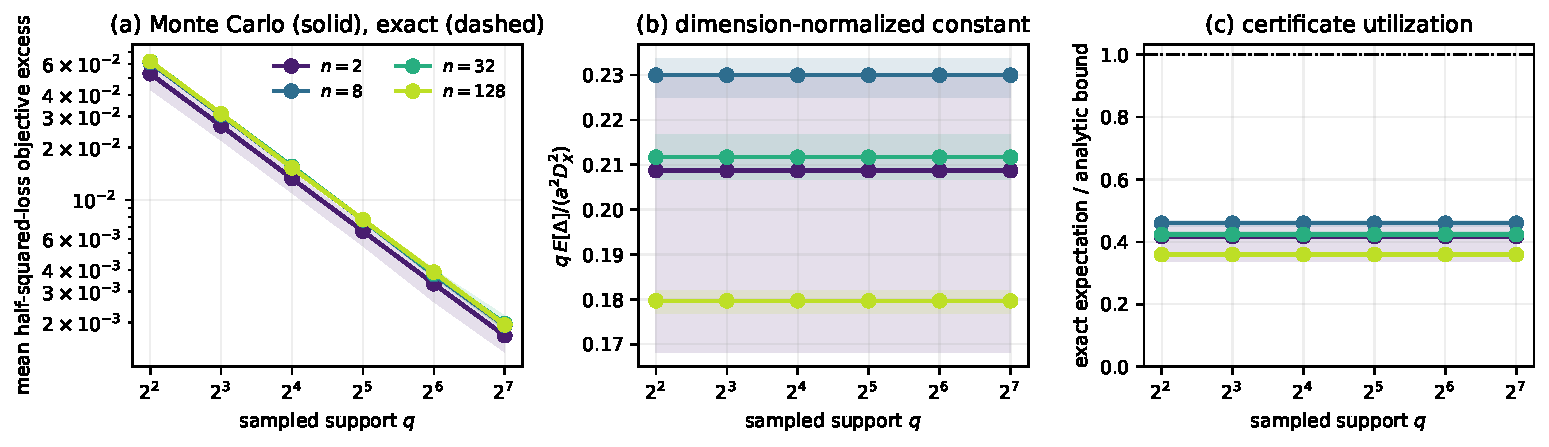
\includegraphics[width=\textwidth]{figures/Fig1.pdf}
\caption{Fixed-dictionary self-sparsification on dense width-256 endpoints.
Solid curves in (a) are Monte Carlo means and dashed curves are the exact
conditional expectations in \eqref{eq:empirical-exact-sampling}; bands are
the full ranges over eight endpoints. Panel (b) removes the theorem's
$q^{-1}$ scale and the data constant. Panel (c) divides the exact expectation
by the analytic smooth bound; the dash-dotted line is one.  This finite
computation checks the implementation and illustrates the mechanism; it is
not evidence for a barrier lower bound or a uniform population statement}
\label{fig:self-sparsification}
\end{figure}

Across all 192 endpoint--support settings, every one of the 2048 sampled
coefficient vectors has support at most $q$ and preserves the $\ell_1$ mass
to the recorded floating-point precision.  The largest exact-to-bound ratio
is $0.4672$.  After normalization, the complete range is
$q\E_I\Delta/(a^2D_X^2)\in[0.1683,0.2336]$ across input dimensions from two to
128.  The largest relative discrepancy between the Monte Carlo mean and the
closed-form expectation is $0.114$.  Thus the observed dimension changes the
finite covariance constant but does not introduce a different power of $q$.

\begin{table}[t]
\caption{Fixed-dictionary self-sparsification diagnostic. The slope is fitted only as an implementation check; the exact conditional expectation is algebraically proportional to $q^{-1}$. Ranges are over eight dense endpoints and all sampled supports}
\label{tab:self-sparsification}
\centering
\begin{tabular}{rrrr}
\toprule
$n$ & fitted slope & max. bound ratio & range of $q\mathbb E\Delta/(a^2D_X^2)$ \\
\midrule
2 & -1.000 & 0.461 & [0.168, 0.230] \\
8 & -1.000 & 0.467 & [0.225, 0.234] \\
32 & -1.000 & 0.434 & [0.207, 0.217] \\
128 & -1.000 & 0.364 & [0.177, 0.182] \\
\bottomrule
\end{tabular}
\end{table}


The same records also check the transfer in
Theorem~\ref{thm:balancing-retraction}.  The square-root lift
$\theta_i^{\rm raw}=\operatorname{sgn}(a_i)\sqrt{\abs{a_i}}$ and
$w_i^{\rm raw}=\sqrt{\abs{a_i}}u_i$ changes the stored predictions by at most
$4.45\times10^{-16}$ and the regularizer by at most
$1.74\times10^{-18}$.  These are invariant checks, not numerical evidence for
the global deformation-retraction claim.

\subsection{Complementary Complete-Path Stress Test}

We retain one complementary diagnostic from the earlier audit because
self-sparsification is only the endpoint-compression step: the theorem also
uses zero-output relocation, a common reference, and labeled coefficient
transfers.  On finite ridge-teacher distributions in dimensions
$n\in\{1,2,4\}$, ten independent pools contain eight projected-proximal-Adam
solutions at each width $m\in\{8,16,32,64,128\}$.  Three disjoint endpoint
pairs are selected per replicate and level.  The constructive path uses the
earlier deterministic cluster compression, followed by exactly the same
zero-buffer/reference part of the proof.  It is compared with direct
interpolation and a mesh-corrected Dynamic String Sampling (DSS) search.  This
test is therefore evidence that the complete path implementation is coherent,
not a second test of the dimension-free sampling rate.

Every nonconstant segment of the constructive path is coefficient
interpolation at fixed first-layer rows, so convexity makes the largest stored
node value an exact upper bound for that complete continuous path.  The DSS
and direct-interpolation values include the segmentwise mesh correction from
the globally Lipschitz Huber objective.  The selected levels are optimizer
proxies and the returned values are upper bounds for finitely many pairs; no
barrier lower bound or full-sublevel estimate is inferred.

\begin{figure}[t]
\centering
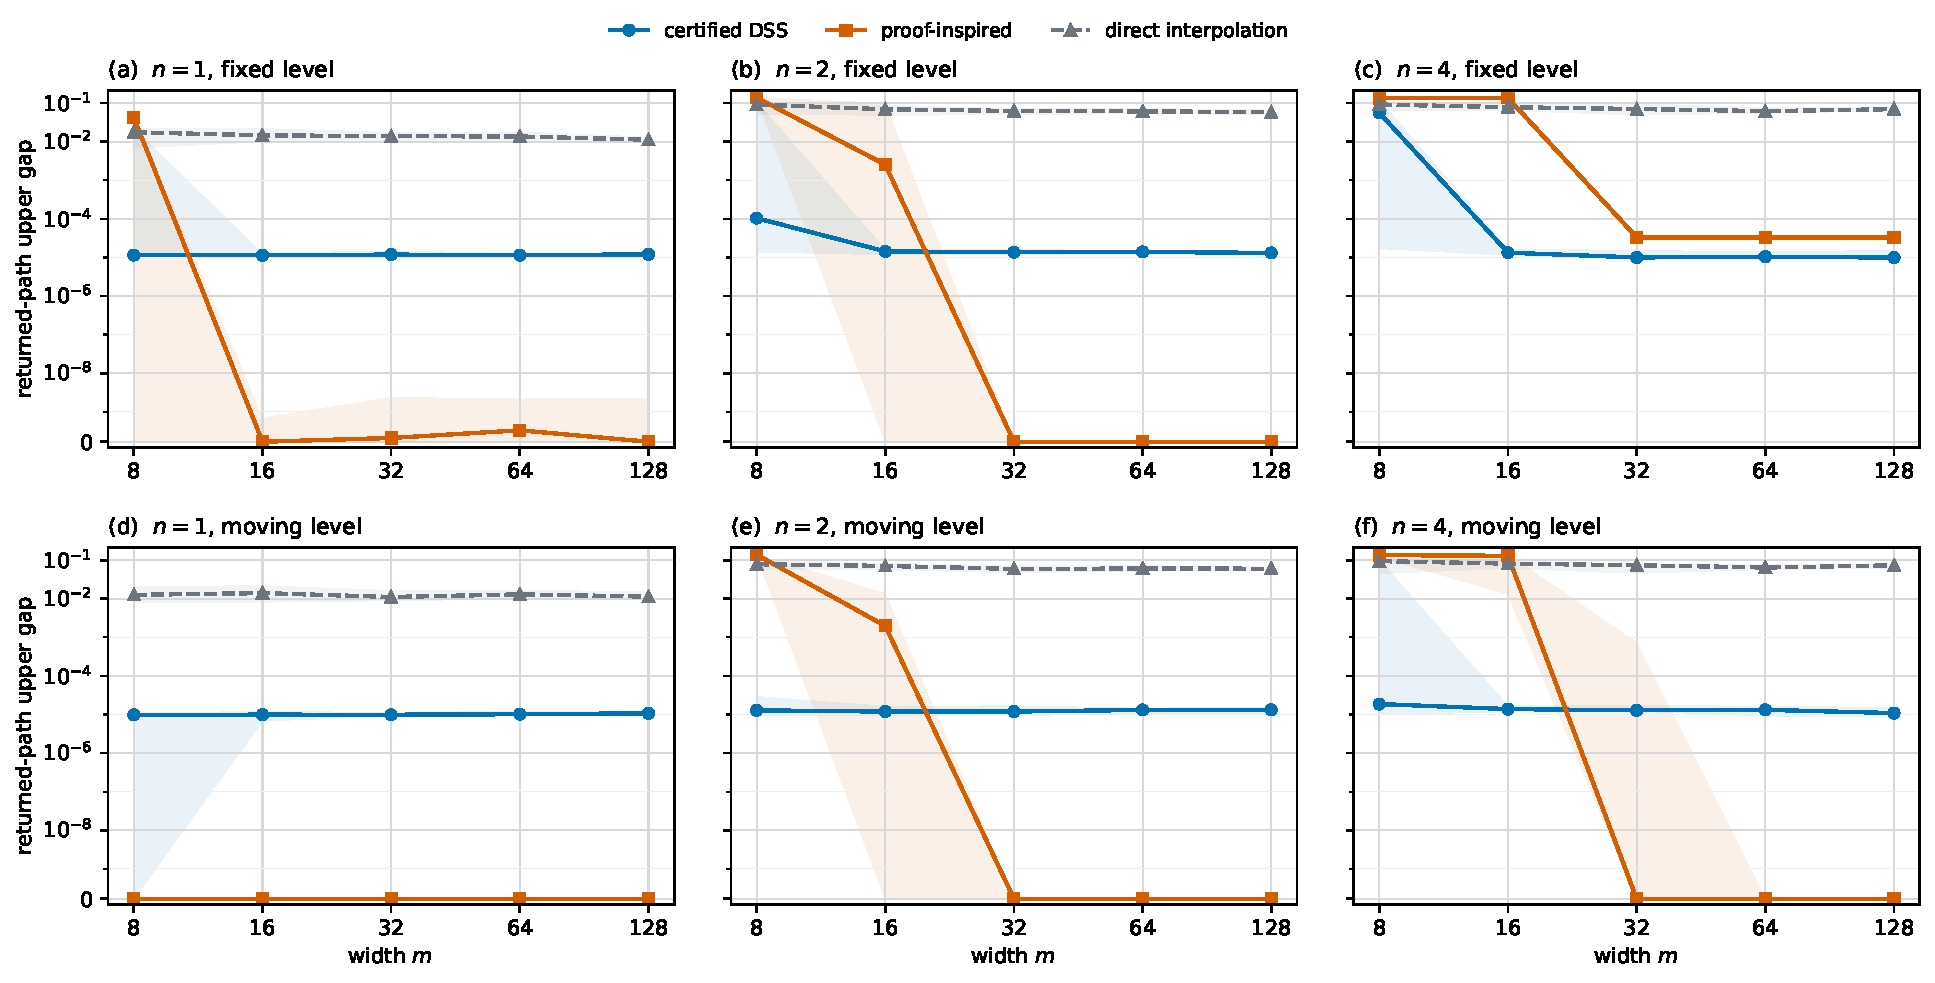
\includegraphics[width=\textwidth]{figures/Fig2.pdf}
\caption{Upper gaps of three complete returned paths. Columns are input
dimensions and rows separate a common fixed level from an optimizer-based
moving level. Each curve is the median of ten replicate-wise maxima over three
disjoint pairs; shading is the full replicate range. The sharp $m=8$ to
$m=16$ transition and the DSS tolerance floor should not be read as a fitted
asymptotic exponent}
\label{fig:path-diagnostics}
\end{figure}

For all 720 recorded Huber pairs with $m\ge16$, the smaller of the certified
DSS and constructive upper gaps is at most $1.6584\times10^{-5}$, or at most
$1.4391\times10^{-3}$ of the selected level.  Direct interpolation is much
higher: its median gap is $4.79\times10^{-2}$.  Table~\ref{tab:main-computation}
separates these finite path observations from the optimization proxy and the
legacy cluster-certificate check.

\begin{table}[t]
\caption{Frozen main-run summary. All path quantities are upper gaps for the recorded endpoint pairs, not estimates of the uniform sublevel barrier. The three path columns use only $m\ge16$; the compression ratio uses all widths. ``Best path'' means the smaller of the certified DSS and exact constructive upper gaps; $B$ is the analytic cluster-merge increment bound}
\label{tab:main-computation}
\centering
\scriptsize
\setlength{\tabcolsep}{3pt}
\begin{tabular}{@{}ccccccc@{}}
\toprule
$n$ & $\widehat e(8)$ & $\widehat e(128)$ & zero constructive & max best-path & median direct/DSS & max $\Delta_{\rm cmp}/B$ \\
 & & & gap (\%) & gap & ratio & \\
\midrule
1 & 0.117451 & 0.117451 & 90.8 & 2.338e-09 & 9.94e+02 & 0.089 \\
2 & 0.023544 & 0.023544 & 90.0 & 1.600e-05 & 4.60e+03 & 0.066 \\
4 & 0.010836 & 0.010721 & 35.8 & 1.658e-05 & 6.10e+03 & 0.045 \\
\bottomrule
\end{tabular}
\end{table}


\medskip
\noindent
Online Resource~1 contains supplementary reproducibility and proof-audit notes,
including frozen experimental parameters, implementation details,
path-certificate definitions, and provenance information.


\section{Discussion and Limitations}\label{sec:discussion}

The main theorem is a statement about constrained one-hidden-layer ReLU networks, expected regularized risk, and scalar logits. The first-layer constraint is essential. With an unrestricted first layer and a penalty only on the output layer, positive homogeneity permits the same predictor to be represented with arbitrarily small regularization cost.

The two loss regimes use genuinely different hypotheses.  The Lipschitz result
allows a risk bounded below and gives an absolute-error estimate.  The
H\"older-smooth result assumes nonnegative loss and integrability at the zero
predictor; these conditions control the atomic mass and justify cancellation
of the first-order term.  Half-squared error is covered by the latter regime,
not by an implicit bounded-logit assumption.

``Dimension-free'' refers to the exponent and to the absence of a covering
number for the first-layer parameter space.  The constant $D_X$ is the
operator-norm second-moment envelope and can itself vary across data
distributions.  The theorem therefore does not claim a universal numerical
constant independent of how the data scale with dimension.

Proposition~\ref{prop:compression-sharpness} is deliberately limited to
same-dictionary compression under a bounded atom envelope.  It neither rules
out faster compression for structured ReLU dictionaries nor supplies a lower
bound for paths that are free to move their atoms.  Establishing sharp
worst-case barrier rates remains open.

Lemma~\ref{lem:maurey} supplies a universal regularized-value rate without a
separate target-class assumption.  Sharper approximation results can improve
constants or rates only after their atom normalization, distribution, loss,
and regularizer have been matched to the present model.

Finally, barrier decay does not by itself imply rapid optimization. The proof constructs an admissible path but gives neither a conditioning estimate nor a guarantee that gradient-based training finds that path.

\section{Conclusions}\label{sec:conclusion}

Fixed-dictionary atomic compression removes the geometric covering bottleneck
from the shallow rectified-linear network path construction. For convex
globally Lipschitz losses, the construction gives inverse-square-root decay
along bounded moving levels, while deterministic smallest-mass pruning gives
inverse-linear decay for every fixed sublevel above the limiting objective.
H\"older regularity of the loss derivative improves the moving-level rate and
reaches inverse-linear decay in the smooth case. A balancing deformation
transfers these results to ordinary two-layer quadratic weight decay without
changing the represented function. The resulting bounds also quantify when
connected components of a lower sublevel merge after a controlled increase of
the objective. The numerical diagnostics support the individual compression,
balancing, and path-construction mechanisms, but the uniform asymptotic
conclusions remain analytic rather than empirical.

\begin{acknowledgements}
The author is grateful to Prof. Dmitry A. Kamaev for valuable discussions and
guidance.
\end{acknowledgements}

\section*{Declarations}

\textbf{Funding.} No funding was received for conducting this study.

\textbf{Competing Interests.} The author declares no competing interests.

\textbf{Ethics Approval.} Not applicable.

\textbf{Consent to Participate.} Not applicable.

\textbf{Consent for Publication.} Not applicable.

\textbf{Data Availability.} No external data are used. Seeded synthetic distributions and frozen records are available under \texttt{v2/results} and \texttt{results} in the public repository.

\textbf{Code Availability.} Reproducibility code, configurations, tests, records, and figure scripts are available under \texttt{v2}, \texttt{theory\_experiments}, and \texttt{results} at \url{https://github.com/Safreliy/energy-gap-estimate}. Historical notebooks remain separate.

\textbf{Author Contribution.} Saveliy Baturin conducted the analysis, implemented the computational diagnostic, and wrote the manuscript.

\bibliographystyle{spmpsci}
\bibliography{bibliography}

\end{document}
